\label{chap:implementation}

Abbildung \ref{fig:data_stream} zeigt die Gesamtübersicht des entwickelten Systems dar. 
\begin{figure*} 
  \begin{center}
    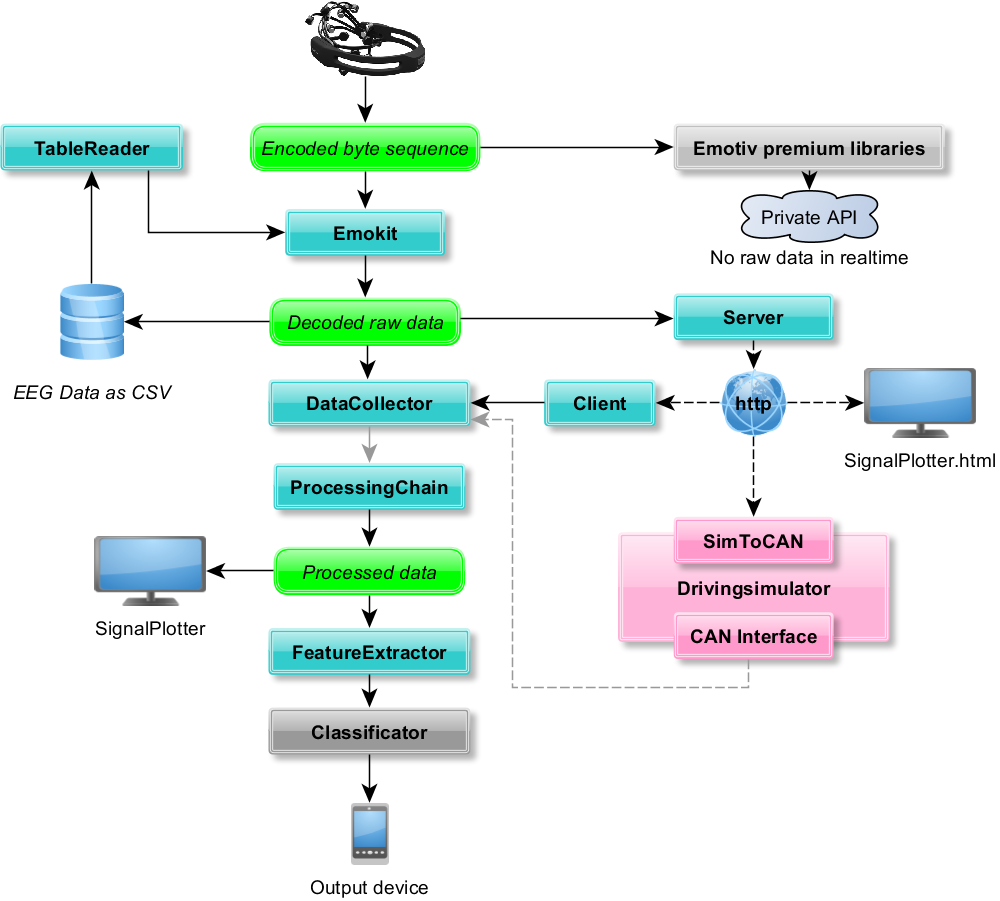
\includegraphics[width=\docwidth]{data_stream}
    \caption[Aufbau der Anwendung]{Der Aufbau des entwickelten System zur Müdigkeitserkennung. Grün: Datenströme, Blau: Python Klassen der Anwendung, Gelb: bedingte Abzweigungen, Rosa: Klassen der Fahrsimulatorumgebung\label{fig:data_stream}}
  \end{center}
\end{figure*}
Alle blauen Klassen der Anwendung wurden in Python 2.7 implementiert. Der Fahrsimulator und seine Schnittstellen (rosa) in Java und C\#, die einzelnen Datenströme sind Grün gekennzeichnet. Bedingte Abzweigungen für alternative Wege in Gelb. Die Anwendung läuft verteilt auf dem DataCollector und dem Embedded PC. Die Datenquelle befindet sich auf dem DataCollector, von dort werden die Daten via CAN-Bus an den Embedded PC übertragen und verarbeitet (Abb. \ref{fig:data_stream_mapping}). 
\begin{figure*} 
  \begin{center}
    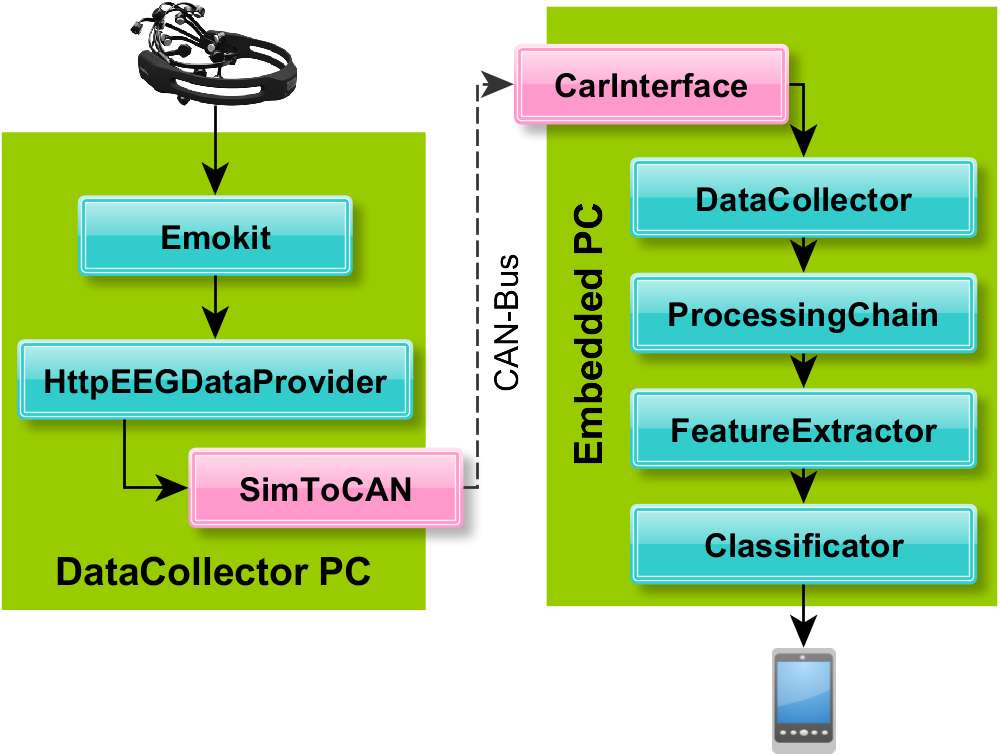
\includegraphics[width=\docwidth]{data_stream_mapping}
    \caption[Einbettung der Anwendung]{Datenquelle und Verarbeitung sind verteilt im Fahrsimulator eingebettet. Die Übertrageung erfolgt via CAN-Bus. \label{fig:data_stream_mapping}}
  \end{center}
\end{figure*}

\threadingSequence

Abschnitt \ref{sec:fetching} befasst sich mit den Rohdaten und deren Weiterreichung im System. Die Verarbeitung der Rohdaten ist Thema von Abschnitt \ref{sec:processing}. Im folgenden Abschnitt werden daraus die passenden Merkmale extrahiert. In Abschnitt \ref{sec:classification} wird die Arbeitsweise des Klassifikators näher beleuchtet. 


